\section{THEORY AND CALCULATION}
\label{sec:theory_and_calculation}
\subsection{Depth Image to Laser Scan}
In this section, the object distance information from the depth image is converted into laser scanning information (sensor\_msgs/msg/LaserScan)~\cite{laserscan}, 
where the information that is important for sensor fusion is:
\begin{itemize}[leftmargin=*]
    \item \textbf{angle\_increment}: The angle between each measurement, 
    which can be used to determine the exact direction of each distance measurement within the scan. 
    \item \textbf{ranges}: A float32 array representing the distance measurement from the scanner to the nearest object for each angle increment. 
    In Gazebo, the LiDAR application is visualised as a circle (or sector) made up of equal parts of laser data slots within a given range (usually $360$ degrees). 
    Two-dimensional laser scanning is typically defined in the plane using polar coordinates, each of which is represented by a distance $r$ and an angle $\varphi$.
\end{itemize}
By default, the centre row of the depth image is used to extract the data that is converted to laser scanning information. 
This maximises the maximum range at which objects can be detected. 
This will be mentioned in the next section: "Trade off in maximum range and object depth". 
Since the goal of this project is to address the disadvantage of LiDAR in detecting low-lying objects, 
the lower part of the depth image is the main focus of the process. 
Therefore, how to convert the coordinates and distance information of any row in the depth image to world coordinates 
so that it can be fused with LaserScan information is the key to this part.

\begin{figure}[H]
    \centering
    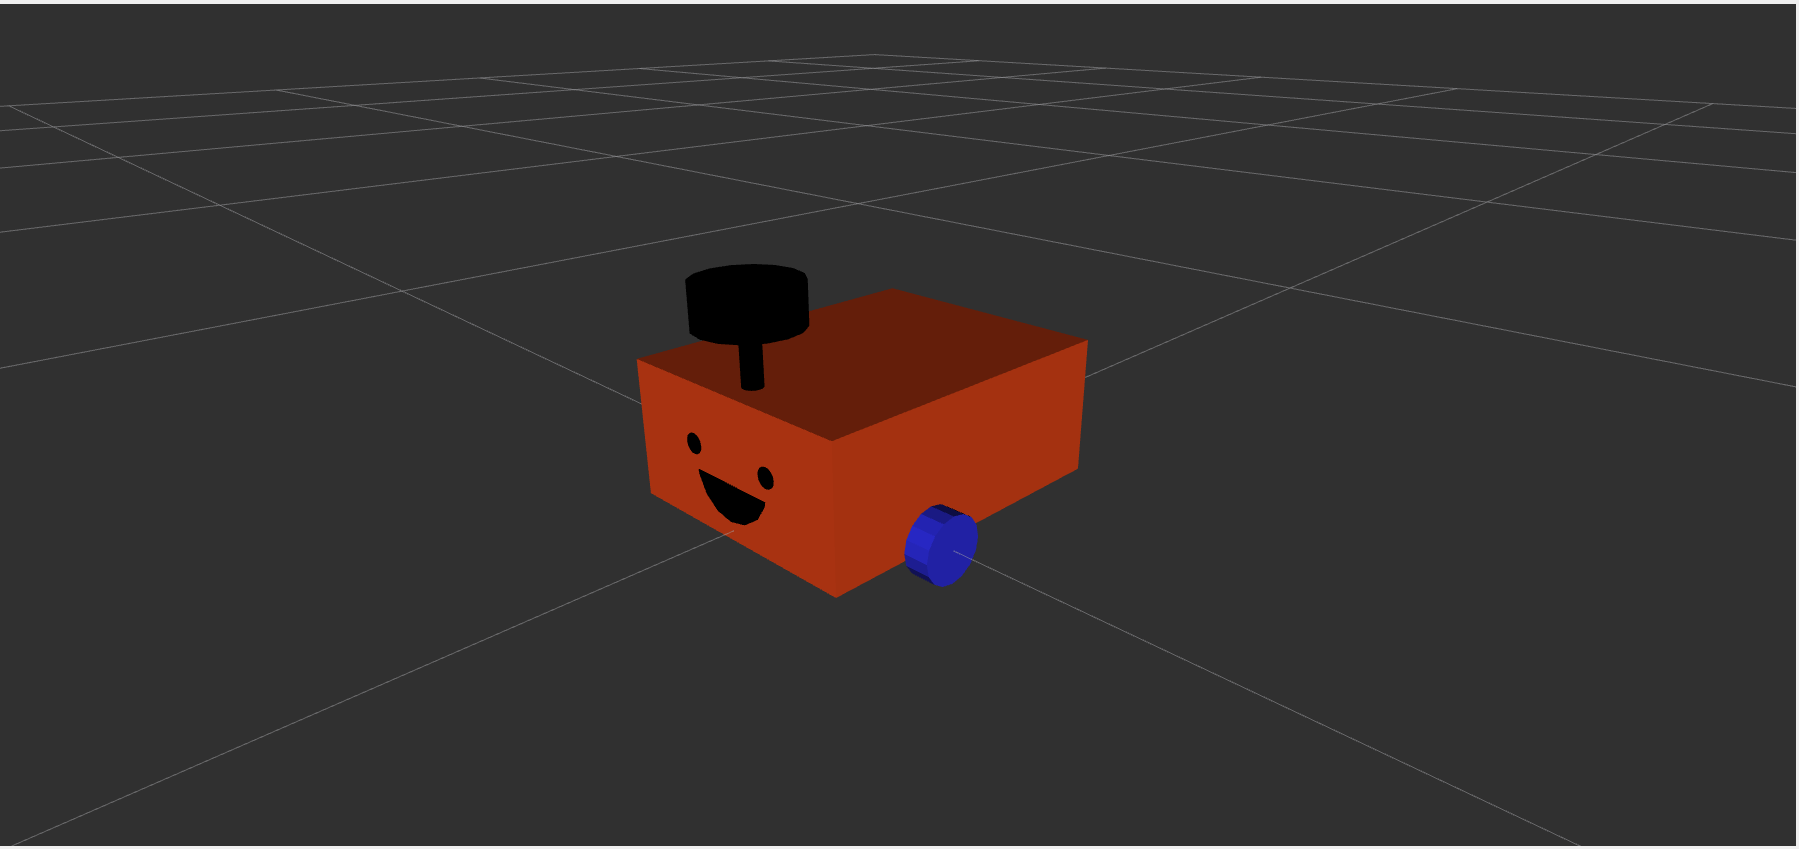
\includegraphics[width=0.8\linewidth]{figs/robot.png}
    \caption{LiDAR visuliaztion in Gazebo}
\end{figure}

A common 2D LiDAR has a resolution of 666, which means that 666 pieces of data will be collected over a 360-degree area. 
A common depth camera produces an image with a resolution of $1920\times1080$ and a field of view of 666 degrees, 
which means that in a selected row, about 666 pixels will be acquired over a 666-degree field of view. 
Therefore, there is no need to worry that the LiDAR data converted from the depth camera data will be limited in the amount of information.

\begin{figure}[H]
    \centering
    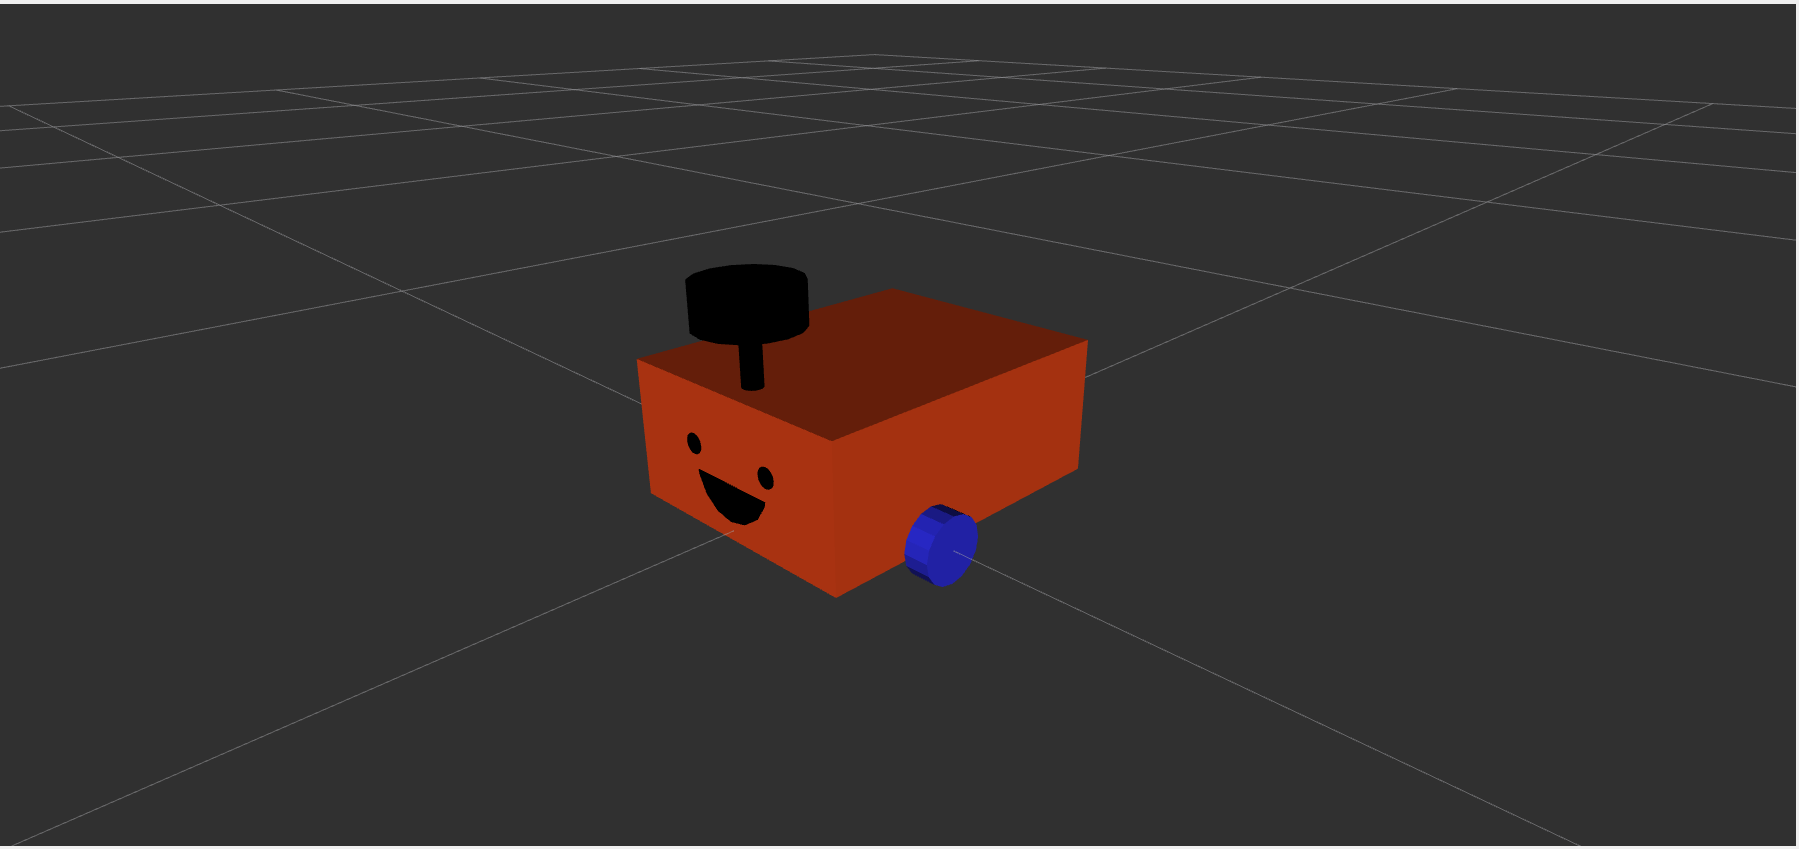
\includegraphics[width=0.8\linewidth]{figs/robot.png}
    \caption{Comparison of depth and normal image}
\end{figure}
In a depth image, the colour of each pixel point represents the distance of this point 
in real-world coordinates from the camera's optical centre. 
Different depth cameras have different ways of colour coding as shown in Figure~\ref{fig:depth_encoding} below.
\begin{figure}[H]
    \centering
    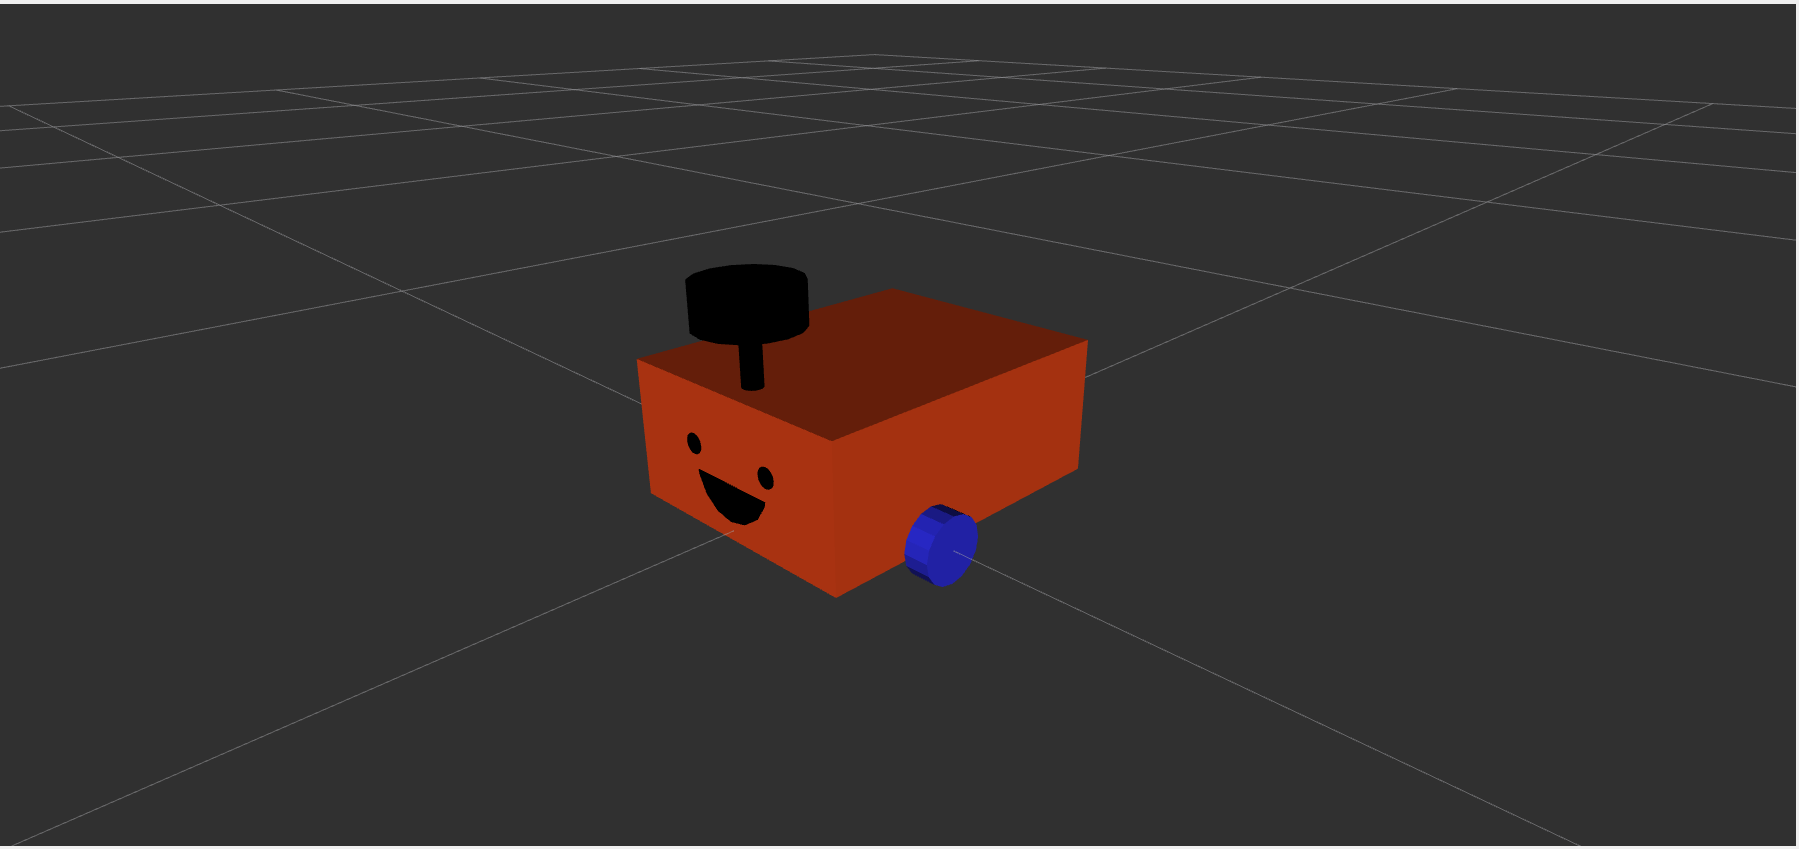
\includegraphics[width=0.8\linewidth]{figs/robot.png}
    \caption{Different depth image encoding methods}
    \label{fig:depth_encoding}
\end{figure}
In this project, depth-gray is chosen as a way to encode distance information in depth images. 
The distance information is expressed in terms of intensity by mapping the depth values to different pixel intensities.
The further away the object is, the lighter the shadow will be. 
Also, since the resolution of the depth image is known ($1920\times1080$ used in this project), the coordinates of any point in the image can be easily represented.
Thus, from the depth map it is known: 
1. the coordinates $p(x, y)$ of the desired point on the image. 
2. the distance from the camera origin $O_c$ to the plane where the object is located, $Z_c$, which is the depth value mentioned above. 
3. the focal length, $f$. These are indicated in following Figure~\ref{fig:depth_coordinate}.
\begin{figure}[H]
    \centering
    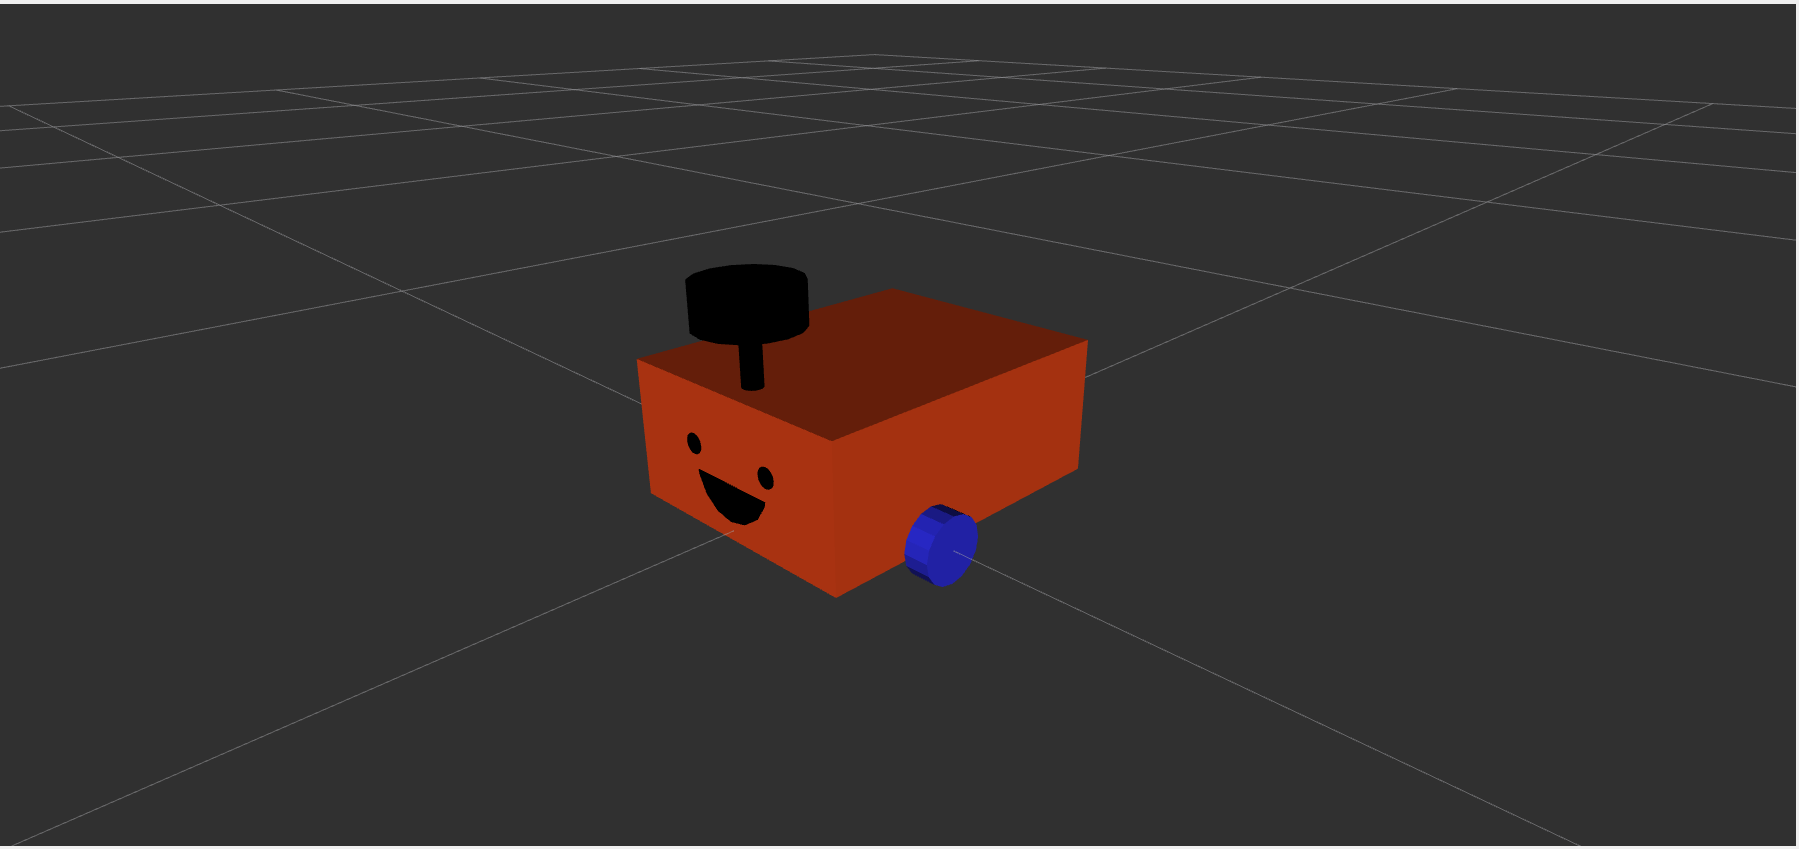
\includegraphics[width=0.8\linewidth]{figs/robot.png}
    \caption{Depth image coordinate system}
    \label{fig:depth_coordinate}
\end{figure}
In order to fuse the depth image data with the LaserScan data, 
the one in the depth image needs to be extracted and processed into the form of laser data slots, i.e. polar coordinates. 
As shown in Figure~\ref{fig:depth_coordinate}, the camera coordinates $(X_c, Y_c, Z_c)$ of point $P$ and its world coordinates $(X_w, Y_w, Z_w)$ 
can be found according to the principle of triangle similarity. 
Then the projection angle of the coordinate point, i.e., the angle $AO_cB$ between the lines $AO_c$ and $BO_c$, can be calculated as 
\begin{equation}
    \theta=\arctan{(\frac{x}{z})}
\end{equation}
The next step is to map the angle $AO_cB$ to the corresponding laser data slot. 
The minimum and maximum range $[\alpha, \beta]$ of the converted laser information is set by the range of the camera field of view, 
and this range is subdivided into $N$ laser data slots, represented by the array $Laser[n]$. 
The index value $n$ of the point $P$ projected to the array $Laser$ can be calculated by Equation~\ref{eq:index}:
\begin{equation}
    n=\frac{\theta-\alpha}{(\beta-\alpha)/N}=N\times\frac{\theta-\alpha}{\beta-\alpha}
    \label{eq:index}
\end{equation}
The value of $Laser[n]$ is the distance $r$ from the point $B$ projected 
by the point $P$ on the $X_cO_cZ_c$ plane to the centre of the camera's optical center $O_c$, 
which can be calculated by Equation~\ref{eq:distance}:
\begin{equation}
    Laser[n]=r=O_cB=\sqrt{Z_c^2+X_c^2}
    \label{eq:distance}
\end{equation}

The above calculation of index values can be quickly understood by a simplified example. 
Assuming that there are $N=4$ laser data slots in a max range $60$ degree and min range $-60$ degree, 
the index of each data slot is shown in following Figure~\ref{fig:laser_index}.

\begin{figure}[H]
    \centering
    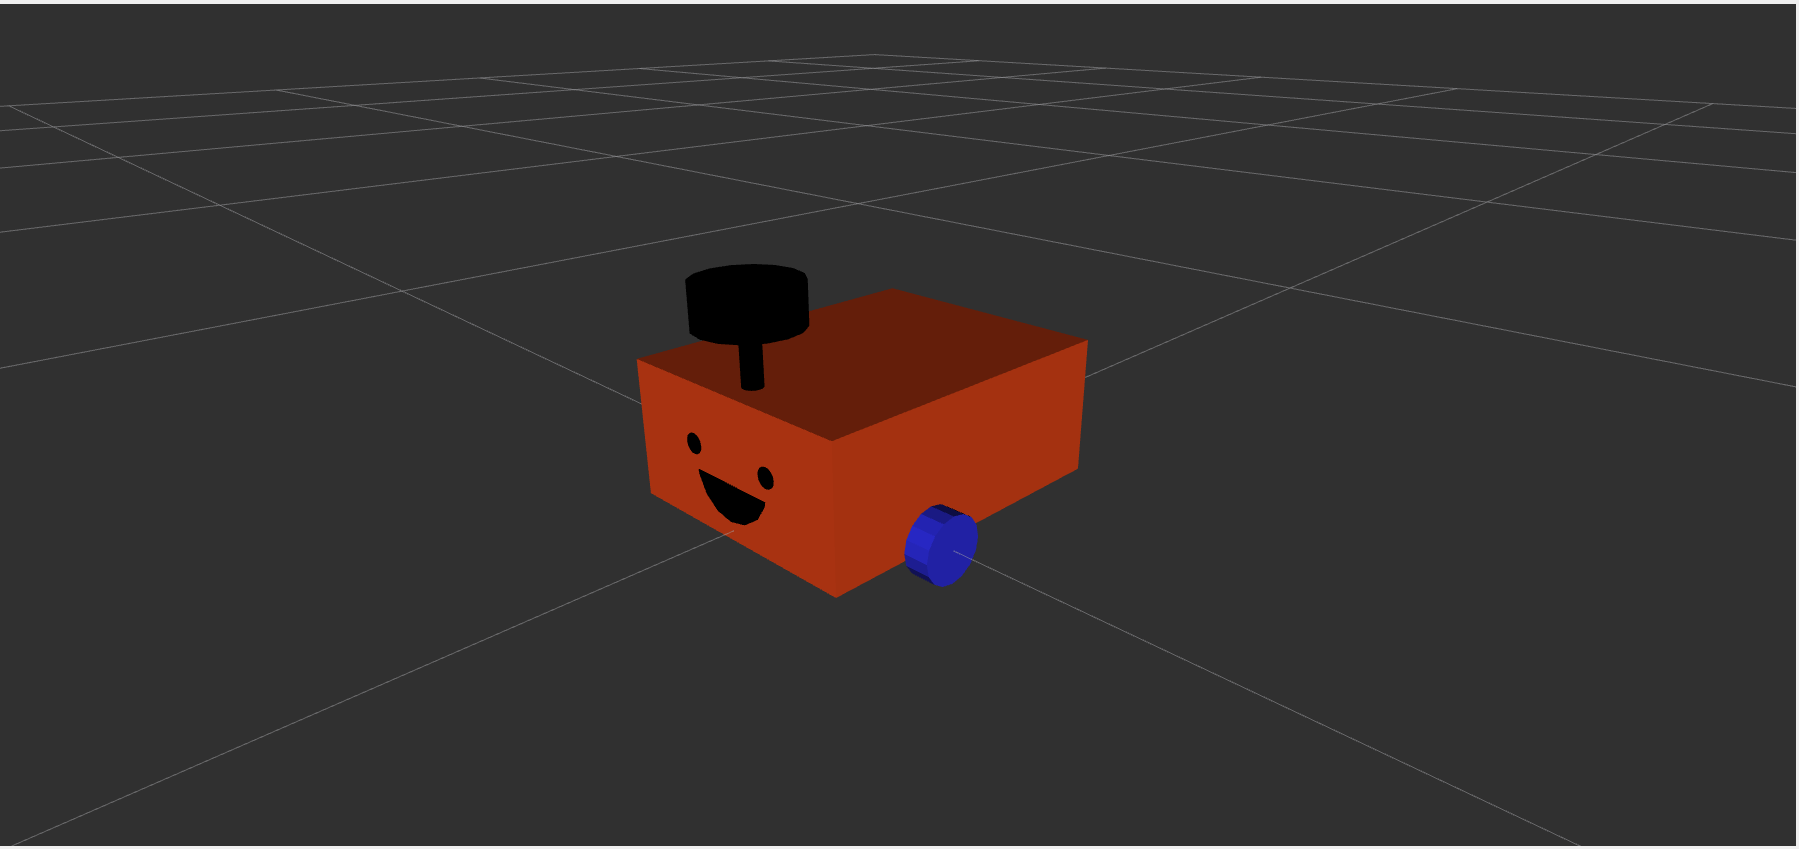
\includegraphics[width=0.8\linewidth]{figs/robot.png}
    \caption{Simplified example of laser data slot index}
    \label{fig:laser_index}
\end{figure}
In order to calculate the index of the laser slot at the 30 degree position, there is: 
\begin{equation*}
    n=N\times\frac{\theta-\alpha}{\beta-\alpha}=4\times\frac{30^\circ-(-60^\circ)}{60^\circ-(-60^\circ) }=3
\end{equation*}
And the logic in coding for this part is shown in the following Algorithm~\ref{alg:Dep2Laser}.
\begin{algorithm}[H]
    \caption{Depth image to LaserScan}\label{alg:Dep2Laser}
    \begin{algorithmic}
    \Require $depth\_image$
    \Ensure A converted LaserScan message from one line of depth image

    \State \textbf{Variables:} scan\_time, range\_min, range\_max, scan\_height, output\_frame\_id
    
    \State \textbf{Initialize} class variables \textbf{with} provided parameters

    \Function{magnitude\_of\_ray}{ray}
        \State \Return $\sqrt{ray.x^2 + ray.y^2 + ray.z^2}$
    \EndFunction
    
    \Function{angle\_between\_rays}{ray1, ray2}
        \State dot\_product $\gets ray1.x \cdot ray2.x + ray1.y \cdot ray2.y + ray1.z \cdot ray2.z$
        \State magnitude\_1 $\gets$ \Call{magnitude\_of\_ray}{ray1}
        \State magnitude\_2 $\gets$ \Call{magnitude\_of\_ray}{ray2}
        \State \Return $\arccos(\frac{dot\_product}{magnitude1 \cdot magnitude2})$
    \EndFunction
    
    \Function{use\_point}{new\_value, old\_value, range\_min, range\_max}
        \State new\_finite $\gets$ isfinite(new\_value)
        \State old\_finite $\gets$ isfinite(old\_value)
        \If{not new\_finite and not old\_finite}
            \State \Return not isnan(new\_value)
        \EndIf
        \State range\_check $\gets$ (range\_min $\leq$ new\_value $\leq$ range\_max)
        \If{not range\_check}
            \State \Return false
        \EndIf
        \If{not old\_finite}
            \State \Return true
        \EndIf
        \State \Return (new\_value $<$ old\_value)
    \EndFunction
    

    
    \end{algorithmic}
\end{algorithm}

\subsection{Tradeoff in Maximum Range and Object Depth}
\label{subsec:tradeoff}
In order to maximise the maximum distance at which objects could be detected, 
the centre row of the depth image was used to extract the data converted to LaserScan information. 
This is due to the fact that although it was implemented to extract any row of the depth image to be converted to LaserScan data, 
the selection of non-centre rows can cause the algorithm to incorrectly consider the floor (or ceiling if taking the top half of the depth image) 
as an obstacle for long maximum range. This will result in the map not being constructed correctly. 
The simulation in RViz2 for this particular situation is shown in Figure~\ref{fig:floor_obstacle}.
\begin{figure}[H]
    \centering
    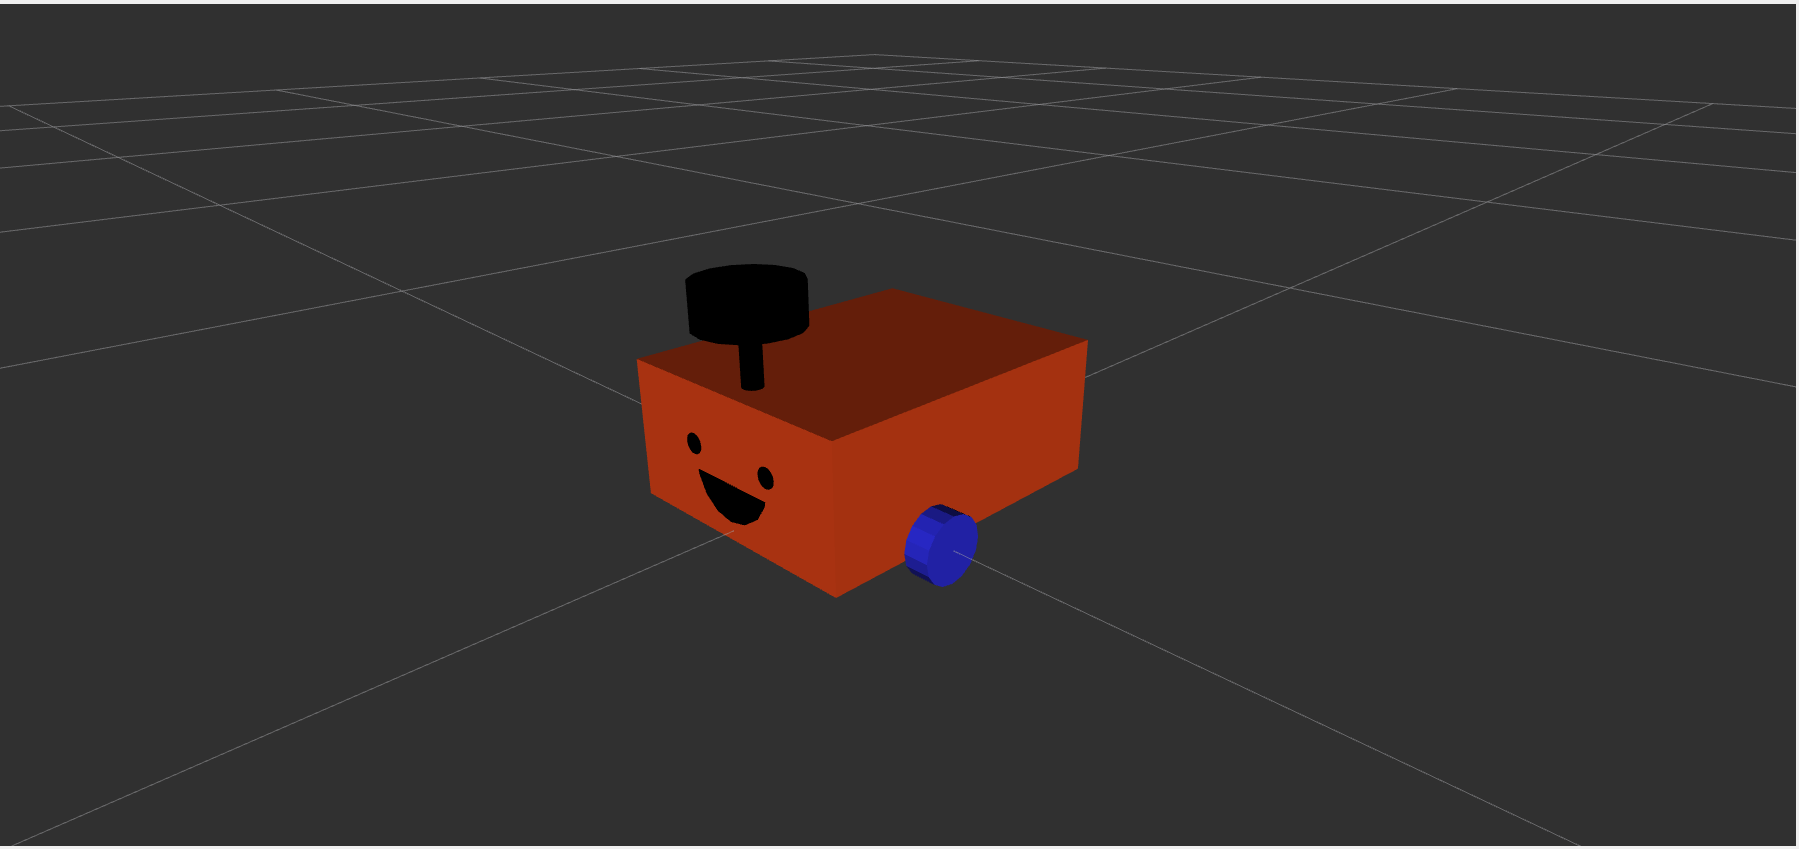
\includegraphics[width=0.8\linewidth]{figs/robot.png}
    \caption{Situation of LiDAR considering the floor as an obstacle}
    \label{fig:floor_obstacle}
\end{figure}
As the aim of this project is to address the disadvantage of LiDAR on low lying objects, 
the lower the obstacle that can be detected is the better, 
therefore selecting the centre horizontal line of the depth image 
and convert it to LaserScan message is not going to maximise the demand. 
The simplest solution is to place the depth camera on a lower position of the robot, 
so that even if the centre line in the image is chosen to be extracted, 
the resulting scanning height is still acceptable. 
However, since this is a hardware solution to the problem, 
it is difficult to implement on different, already assembled robots. 
Algorithm-based approaches are still needed to obtain a generic solution to this problem. 

\begin{figure}[H]
    \centering
    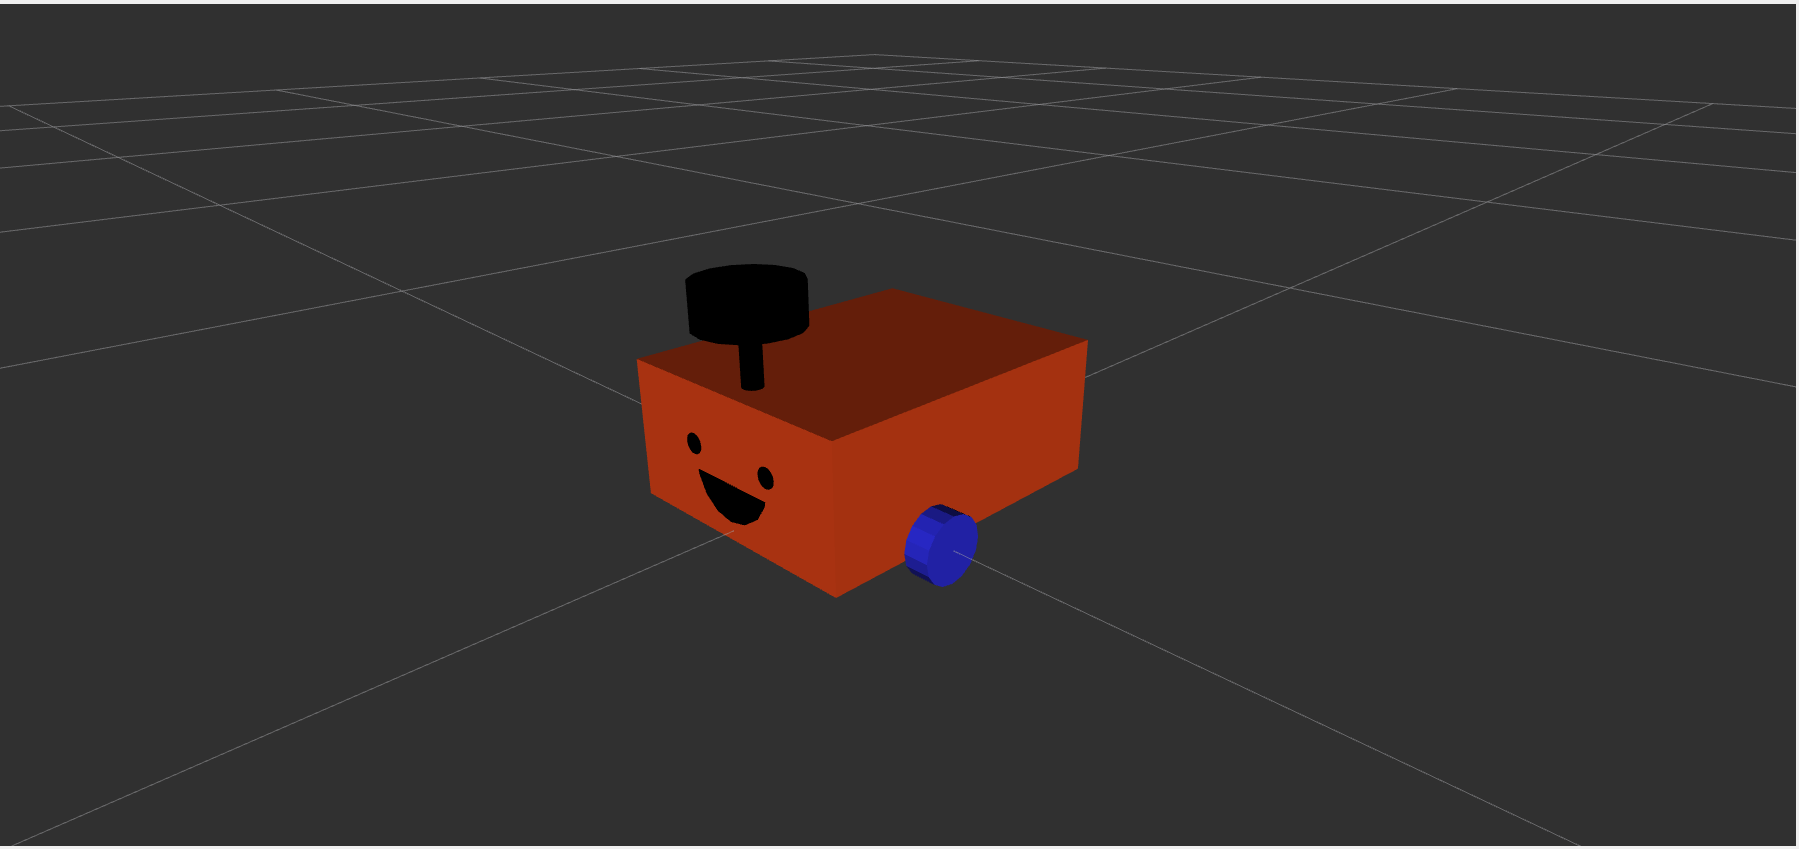
\includegraphics[width=0.8\linewidth]{figs/robot.png}
    \caption{Typical indoor robot with camera on top}
\end{figure}

The Figure~\ref{fig:tradeoff} shows how to calculate the maximum distance $l$ from a point when the chosen horizontal line is offset from the original centre line by $h$, 
which will be uniformly called to as the "line of sight". 
When the line of sight meets the ground, the length of the line of sight is the maximum distance, 
in which case choosing a larger distance would cause the map to fail to be constructed. 
This method therefore ensures that the scan is maximised in a given situation while avoiding the wrong identification. 
Assuming that there is an obstacle close to the ground, 
its horizontal height difference from the depth camera's optical center can be seen as equivalent to the distance $h$ from the depth camera's optical center to the ground.
The angle $\alpha$ is the angle by which the line of sight is offset from the horizontal line at the centre of the frame to the selected horizontal line immediately above the ground. 
At this point it can be seen that the maximum distance $l$ of the original horizontal line of sight is too long and crosses the horizon after a clockwise rotation $\alpha$,
i.e., it will lead to an erroneous situation of judging the ground as an obstacle.

\begin{figure}[H]
    \centering
    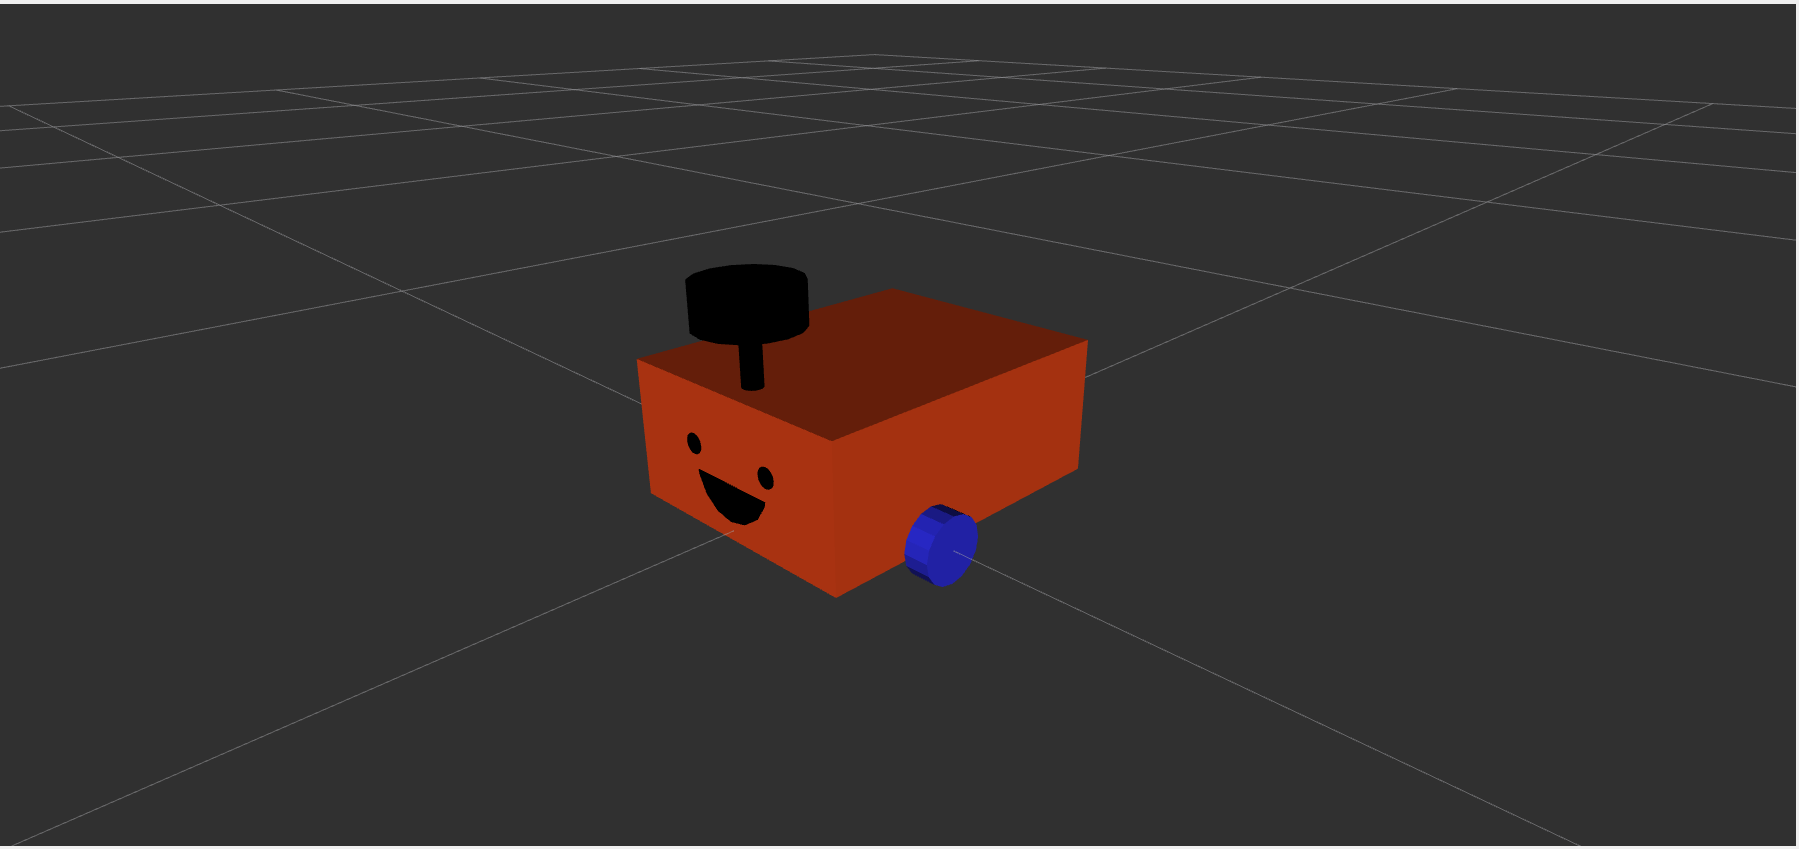
\includegraphics[width=0.8\linewidth]{figs/robot.png}
    \caption{The tradeoff in maximum range and object depth}
    \label{fig:tradeoff}
\end{figure}

In Figure~\ref{fig:tradeoff2}, the maximum distance $l$ in this case is obtained by assuming that after the line of sight is rotated $\alpha$, 
it just intersects the ground. The depth camera optical centre is still at a distance $h$ from the ground. 
Let there be a wall as an obstacle in the horizontal line of sight, the point $p$ is the position 
scanned by the depth camera in the horizontal line of sight, and the point $p'$ is the position 
scanned by the depth camera after the line of sight has been rotated $\alpha$.

\begin{figure}[H]
    \centering
    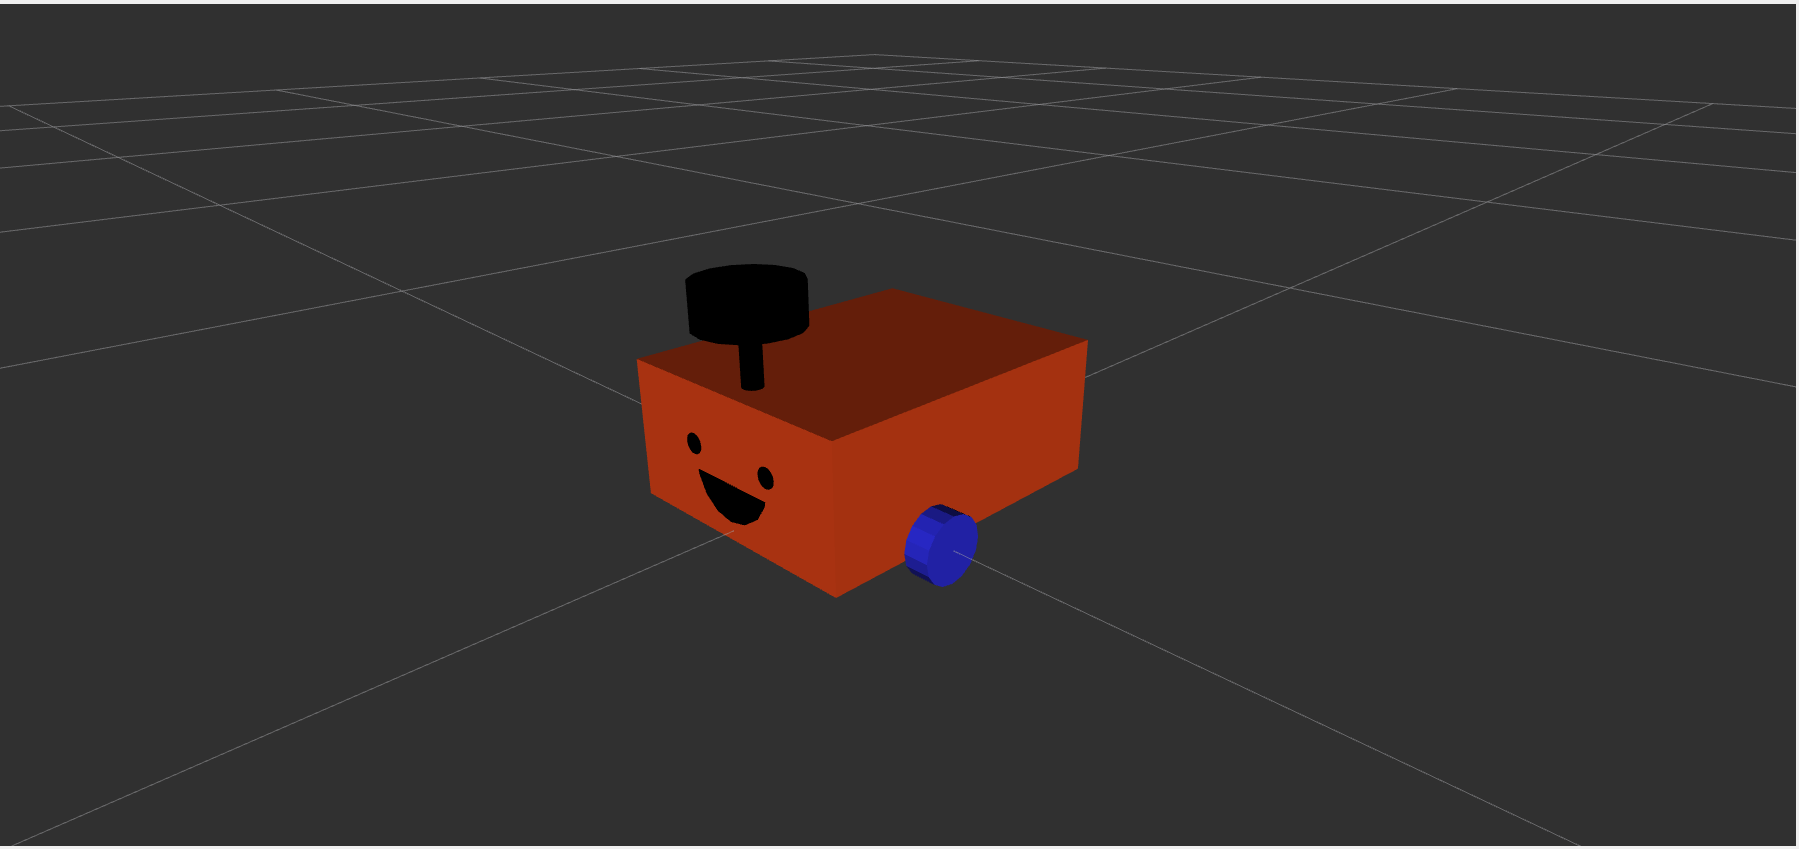
\includegraphics[width=0.8\linewidth]{figs/robot.png}
    \caption{The tradeoff in maximum range and object depth}
    \label{fig:tradeoff2}
\end{figure}

At this point the line of sight is rotated $\delta$ further downwards in order to scan at a lower height. Although it is still possible to scan the obstacle point $p''$ where the wall is lower, the line of sight crosses the horizon, causing an error condition to occur. The length $l'$ of the line of sight that does not cross the horizon needs to be calculated so that the problem can be solved by reducing the maximum distance of the line of sight. 
The length $l'$ of the line of sight that does not cross the horizon can be calculated by equation~\ref{eq:tradeoff} below 
\begin{equation}
    l'=\frac{h}{\sin{(\alpha+\beta)}}
    \label{eq:tradeoff}
\end{equation}
where $\alpha+\beta$ can be expressed as $\arctan(\frac{h'+x}{c})$. 

The reduction in scanning height $h'$ caused by the line-of-sight rotation $\alpha$ can be expressed as, $\tan\alpha=\frac{h'}{c}
$, since $\sin\alpha=\frac{h}{l}$. The angle $\alpha$ can be expressed as $\alpha=\arcsin(\frac{h}{l})$, which gives
\begin{equation}
    h'=\tan(\arcsin(\frac{h}{l}))\times c
\end{equation}
Finally, substituting into the original equation yields: 
\begin{equation}
    l'=\frac{h}{\sin{(\arctan(\frac{\tan(\arcsin(\frac{h}{l}))\times c+x}{c}))}}
\end{equation}
where $l'$ is the new max range after tradeoff. Define it into the programme, it can be seen that the error was fixed successfully.

\begin{figure}[H]
    \centering
    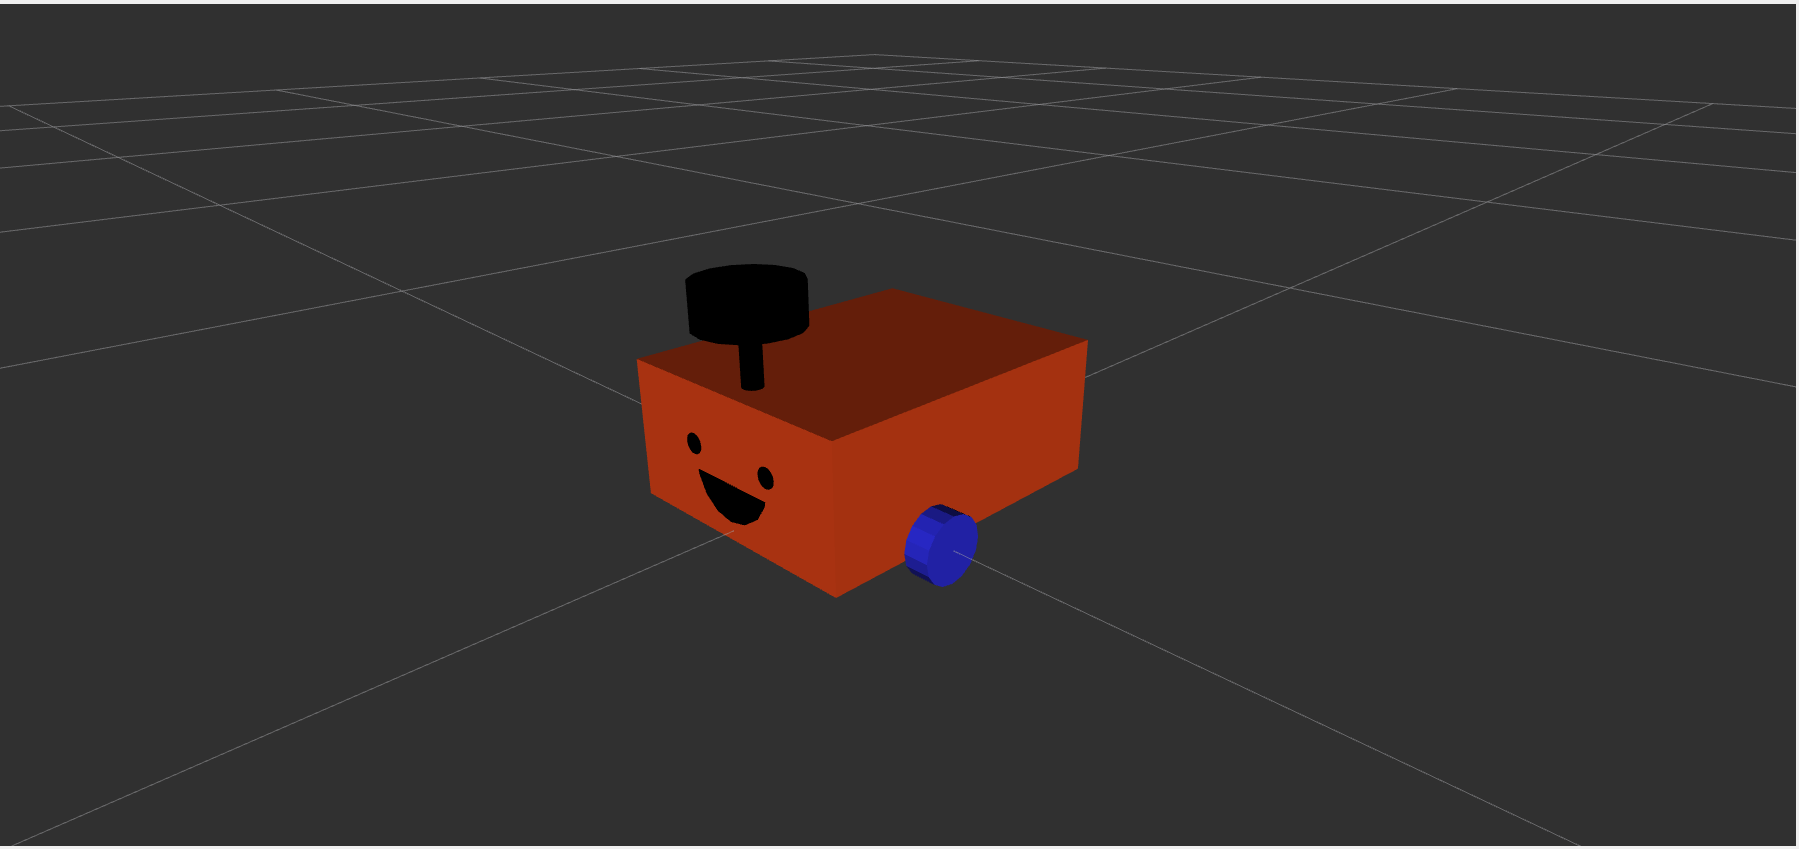
\includegraphics[width=0.8\linewidth]{figs/robot.png}
    \caption{The same situation after fixed}
\end{figure}

Furthermore, from the representation of the diagonal $\alpha$ above, 
it can be seen that $\alpha$ can be represented by an inverse $\sin$ wave which is a positively proportional function. 
It confirms that the more the line of sight is offset downward from the centre horizon, 
the greater the maximum detection distance sacrificed. 
Although adjusting the height of the depth camera from the hardware is not recommended, 
if the depth camera is placed too high, the maximum detection distance sacrificed will be large, 
thus significantly reducing the effectiveness of this fusion algorithm. 
Therefore it is necessary to reduce the height of the depth camera even though the algorithm can be adjusted to detect objects in lower lying areas of the field of view.

\subsection{Merge of LaserScan data and Depth Image Data}
By the above method, the obstacle information 
within a reasonable range in any row within the depth camera's field of view can be obtained and presented
in RViz2 as LaserScan data, as shown in Figure~\ref{fig:centre_row} and Figure~\ref{fig:lower_row}.
\begin{figure}[H]
    \centering
    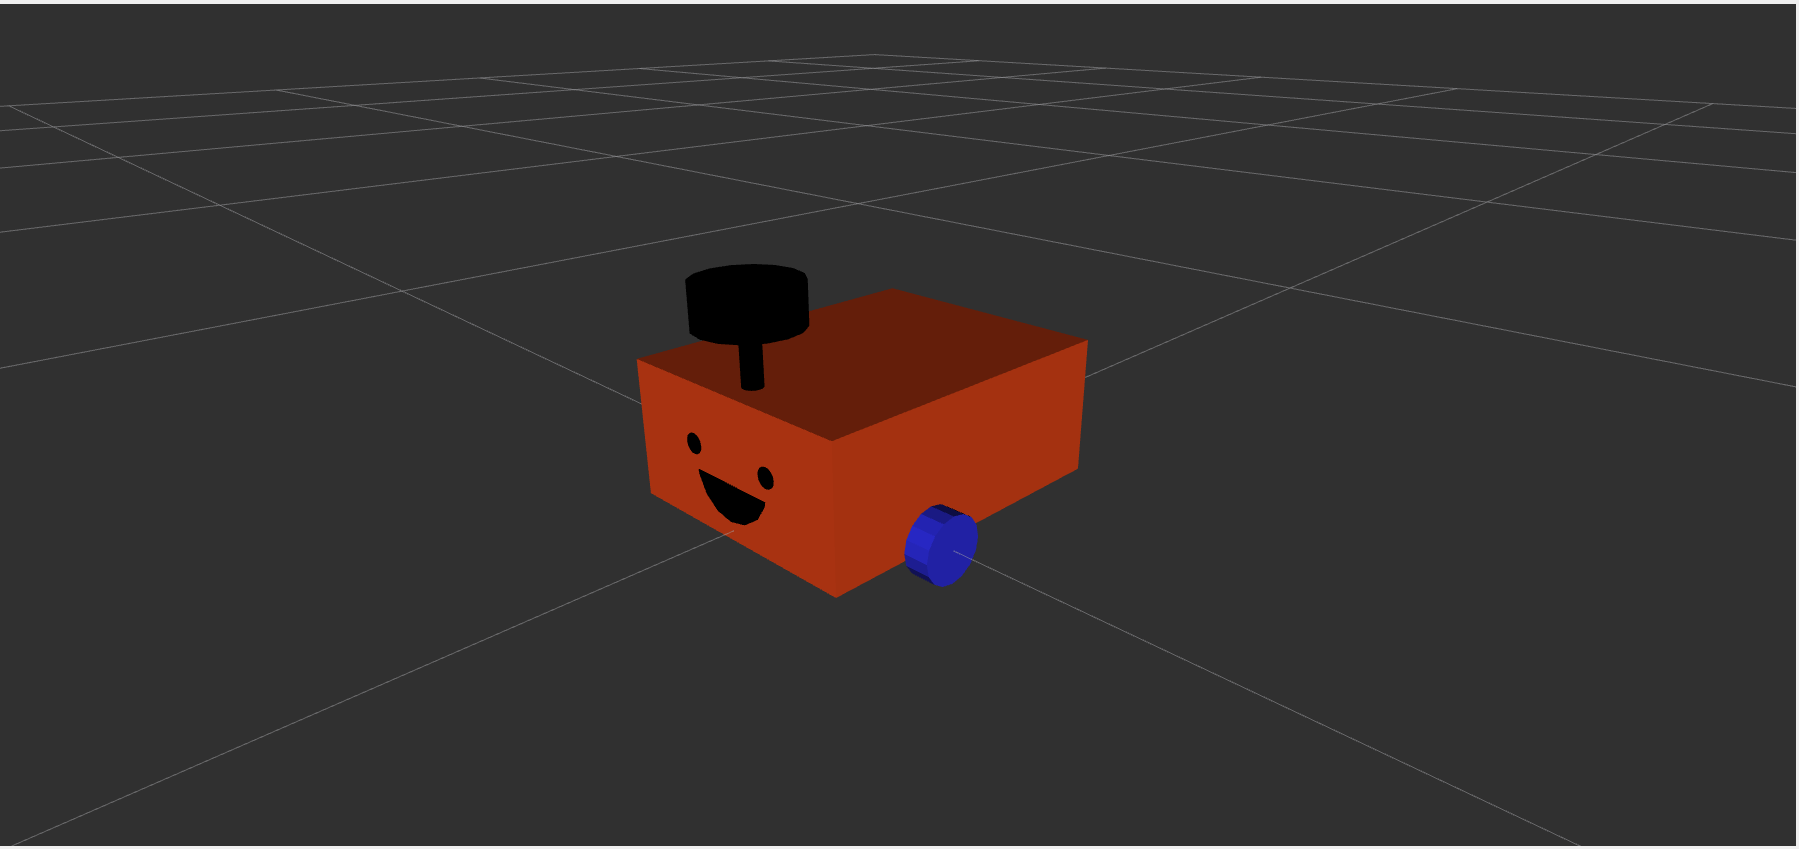
\includegraphics[width=0.8\linewidth]{figs/robot.png}
    \caption{Converted LaserScan data from depth image using the center row}
    \label{fig:centre_row}
\end{figure}
\begin{figure}[H]
    \centering
    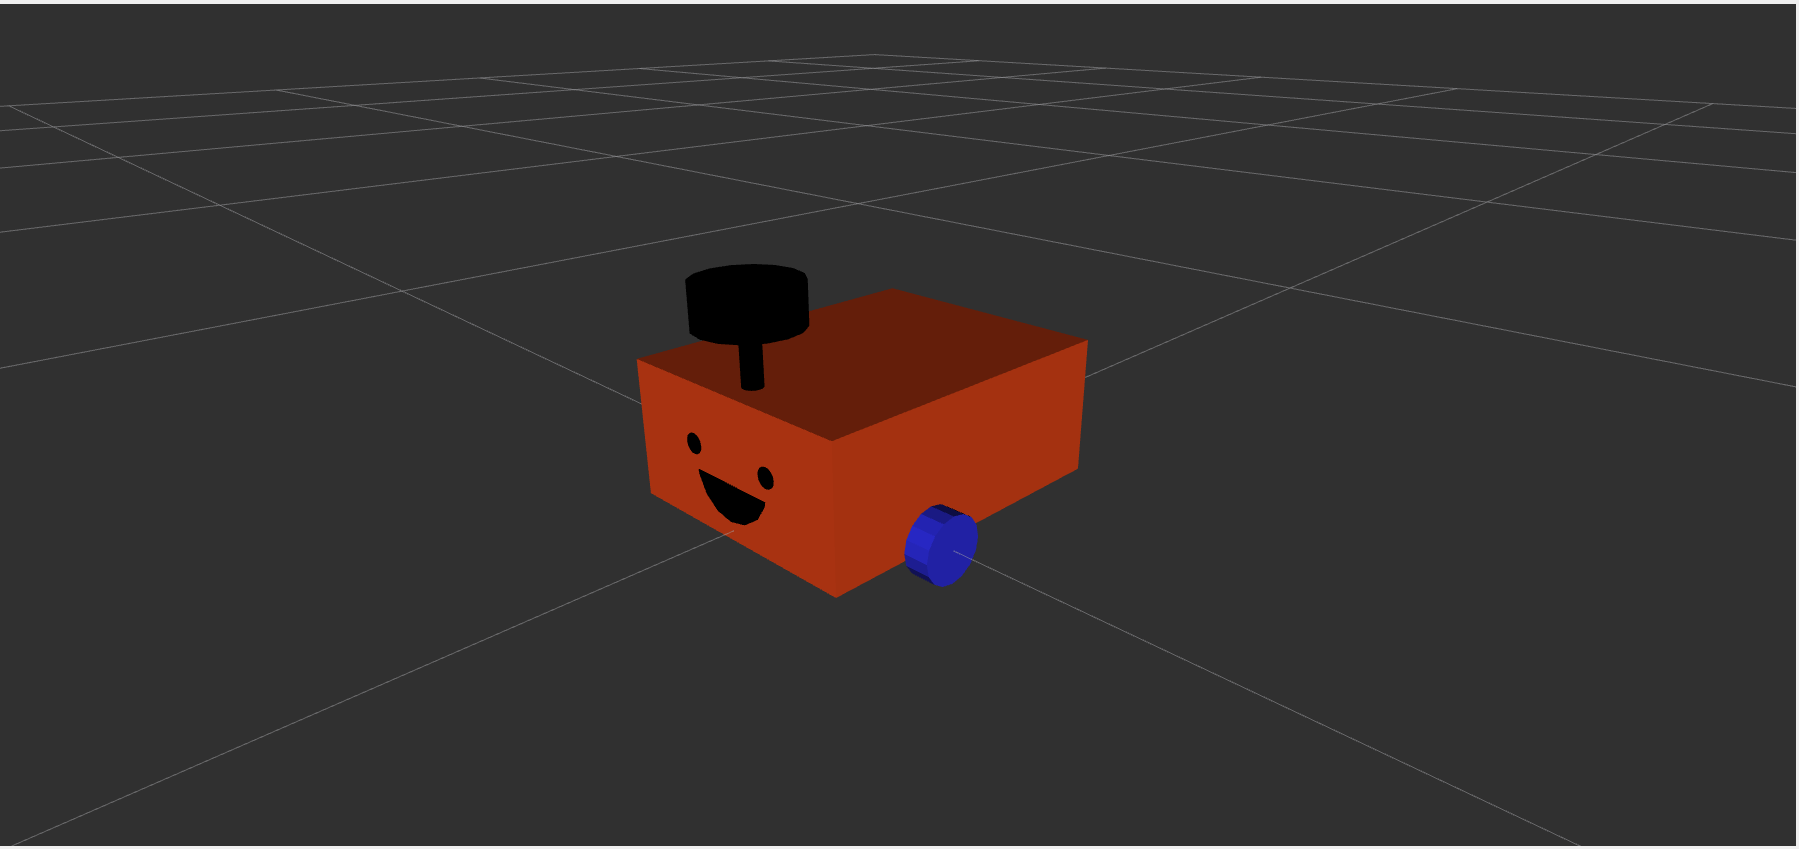
\includegraphics[width=0.8\linewidth]{figs/robot.png}
    \caption{Converted LaserScan data from depth image using the lower row}
    \label{fig:lower_row}
\end{figure}
The author of slam\_toolbox points out that this package does not support multi-laser configs, 
so two sets of lidar information must be combined into one. 
Although the author suggests a solution: use the laser\_assembler package~\cite{github}.
However, this package is not well ported for ROS2
and has problems with not working properly or performing a lot of unnecessary calculations in tests. 

Therefore, a simple and efficient fusion method is designed for this project. 
There are two sets of LiDAR data, one with a range of 360 degree and one with a range of $[\alpha,\beta]$ converted from depth images. 
These two sets of LiDAR data are not at the same height, but this is not important in the 2D map, as shown in Figure~\ref{fig:lidar_scan} and Figure~\ref{fig:depth_scan}.
\begin{figure}[H]
    \centering
    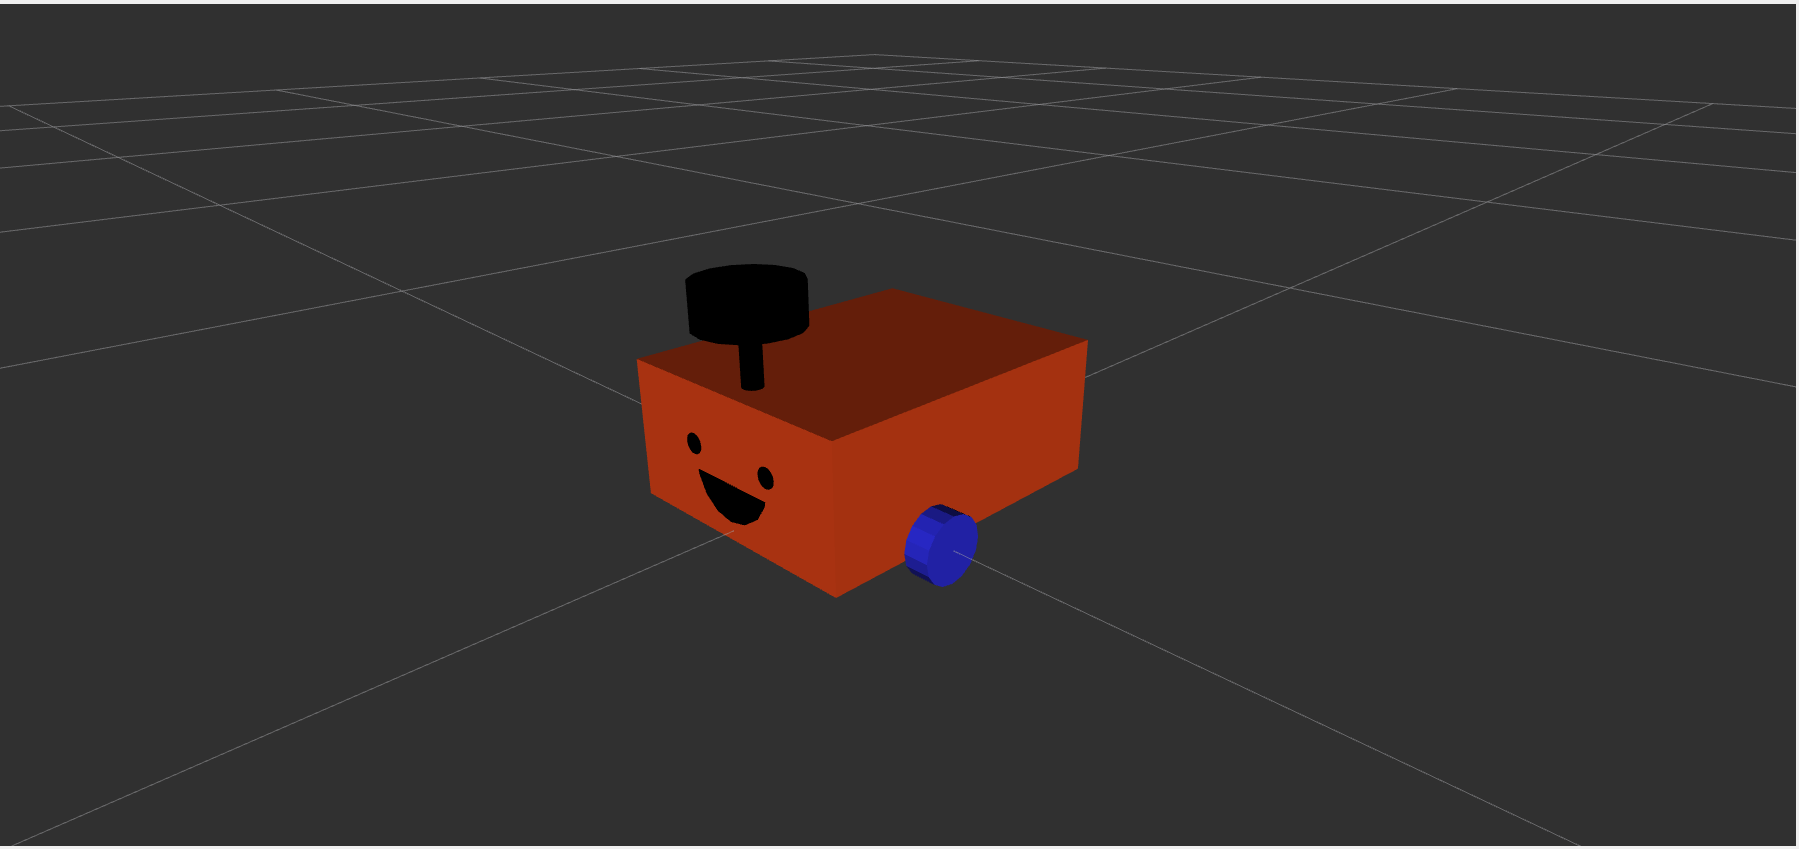
\includegraphics[width=0.8\linewidth]{figs/robot.png}
    \caption{Scan range of LiDAR}
    \label{fig:lidar_scan}
\end{figure}
\begin{figure}[H]
    \centering
    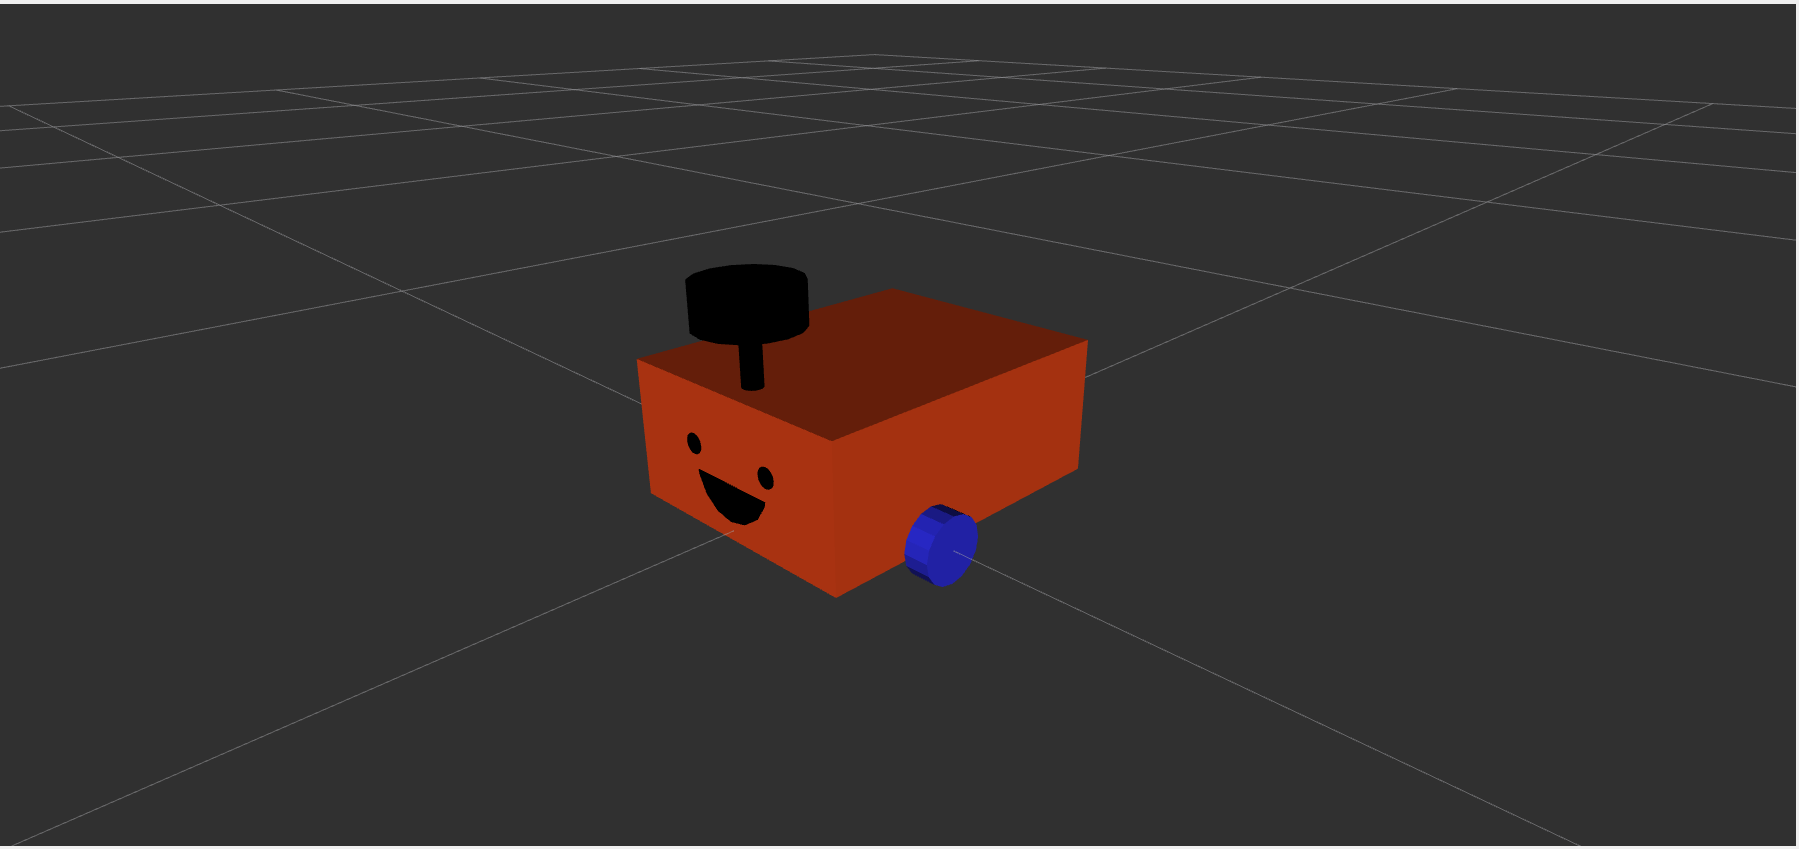
\includegraphics[width=0.8\linewidth]{figs/robot.png}
    \caption{Scan range of depth image}
    \label{fig:depth_scan}
\end{figure}
A new dummy LaserScan array is created. And since there is more LaserScan data with a larger range, 
the $range$ values are compared at the location where the two sets of data overlap, 
based on the LaserScan resolution. The smaller value, which is the closer obstacle, 
is entered into the dummy array. The logic of this part is shown in the following Algorithm~\ref{alg:scan_merge}.

\begin{algorithm}[H]
    \caption{Merge two LaserScan messages into one}\label{alg:scan_merge}
    \begin{algorithmic}
    \Require $lidar\_msg$ , $depth\_msg$ \Comment{LaserScan messages from LiDAR and depth image}
    
    \Ensure A merged LaserScan message with the minimum ranges from both inputs
    \State \textbf{Initialize} merged ranges list: $merged\_ranges \gets [\,]$
    \For{$index = 0$ \textbf{to} $\text{length of } lidar\_msg.ranges$}
        \State $range_l \gets lidar\_msg.ranges[index]$
        \State $range_d \gets depth\_msg.ranges[index]$
        \State \textbf{Append} $\text{min}(range_l, range_d)$ \textbf{to} $merged$
    \EndFor

    \State \textbf{Create} a new LaserScan message $merged$ \textbf{with}
        \State $header \gets$ lidar.header
        \State $angle\_min \gets$ lidar.angle\_min
        \State $angle\_max \gets$ lidar.angle\_max
        \State $angle\_increment \gets$ lidar.angle\_increment
        \State $time\_increment \gets$ lidar.time\_increment
        \State $scan\_time \gets$ lidar.scan\_time
        \State $min \gets$ min(lidar.range\_min, depth.range\_min)
        \State $max \gets$ max(lidar.range\_max, depth.range\_max)
        \State ranges $\gets merged$

    \State \textbf{return} merged
    \end{algorithmic}
\end{algorithm}

In this way, the algorithm automatically determines the greater range of obstruction for the same obstacle, 
regardless of whether the obstacle is more obstructed at a lower or higher location. 
The fusion of the two LaserScan information does not affect the information returned by the original LiDAR.

\subsection{Resample of Depth Image Data}
However, the fusion of the two LaserScan messages in the previous section is not ideal, as shown in Figure~\ref{fig:fusioned}.
\begin{figure}[H]
    \centering
    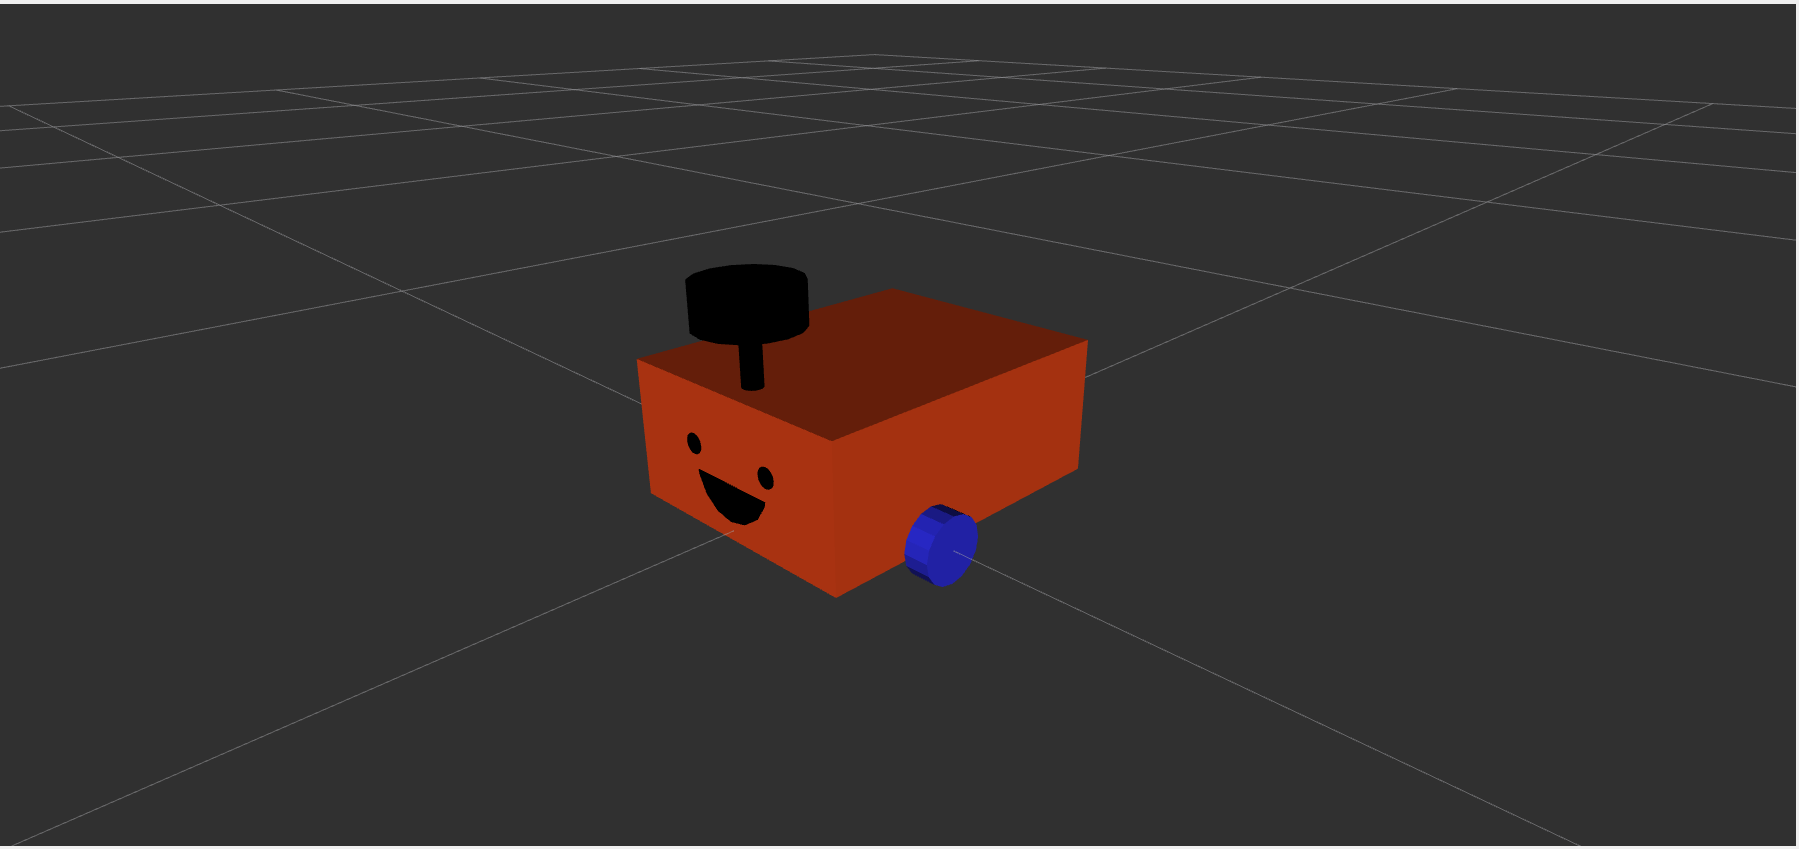
\includegraphics[width=0.8\linewidth]{figs/robot.png}
    \caption{Fusioned LaserScan data before resample}
    \label{fig:fusioned}
\end{figure}
This is because the resolution of the LaserScan information converted from LiDAR and depth images is not the same. 
As there are $1024$ pixels per line in a $1920\times1080$ depth image, 
all $1024$ pixels are used to convert to LaserScan information. 
However, there are only about 666 LaserScan data in the overlapping portion of the LiDAR LaserScan information, 
which makes the fusion between the two contradictory.
\begin{figure}[H]
    \centering
    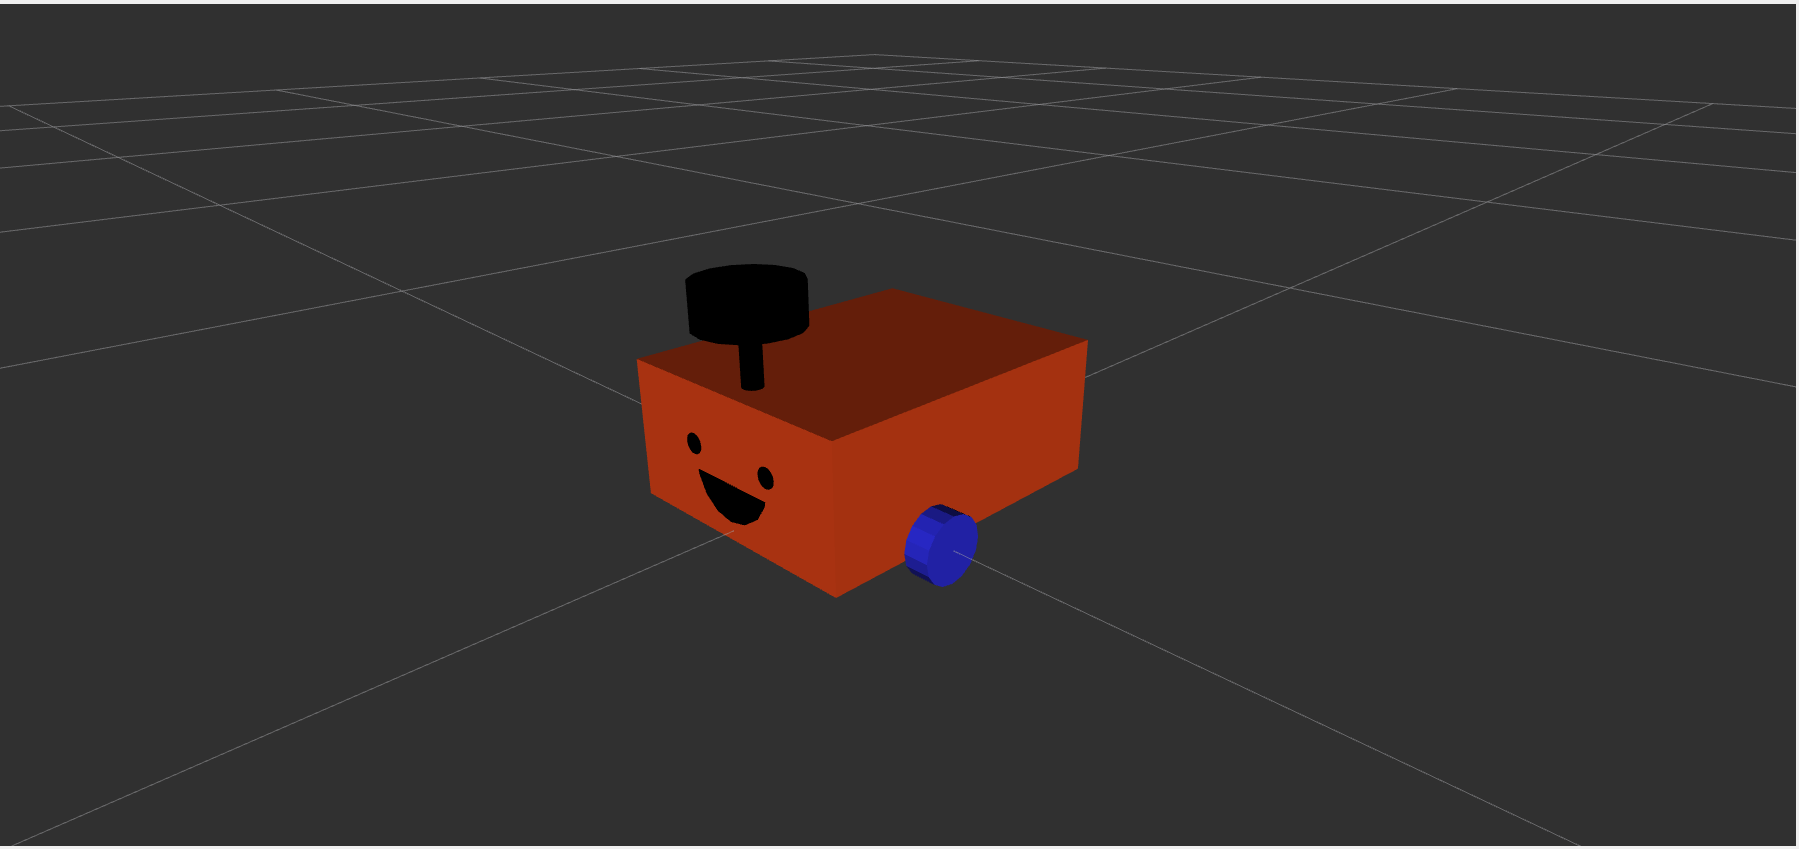
\includegraphics[width=0.8\linewidth]{figs/robot.png}
    \caption{The contradictory in resolution}
\end{figure}
In order to solve this problem without degrading the accuracy of the depth image conversion, 
the resolution of the two LaserScan's need to be harmonised,
based on the data preprocessing in section~\ref{subsec:tradeoff} followed by a Resample operation.

Resample the LaserScan data for depth image conversion. 
First, this method receives two parameters: the original (converted from depth image) LaserScan data, 
and the LaserScan data of the target (LaserScan information from the LiDAR). 
These two sets of data contain, but are not limited to, 
the corresponding angle increments, minimum angle, and maximum angle.

After that, a new LaserScan message is created to store the resampled scan data. 
The header information, time increments, scan time, minimum and maximum ranges of the new scan data 
remain the same as the original scan data, 
while the angular minimum, angular maximum and angular increments are to use the new target values. 
Interpolation is used to obtain the corresponding $range$ values of the target angles.

Then, the angles of the original and target scan data are stored 
in two arrays of values generated at specified intervals within the specified range. 
And then the target angles are interpolated to obtain the corresponding $range$ values. 
The target angle is linearly interpolated based on the original angle and the $range$ value. 
If the target angle is out of the range of the original angle, 
the corresponding $range$ value is set to NaN. finally, the new scan data is returned.

In other words, the new scan data still uses the data converted from the depth image, 
but only the corresponding amount of data that overlaps with the LaserScan data is retained. 
At the same time, the $range$ of the scan is changed to that of the LiDAR LaserScan data (360 degrees), 
except for the portion outside the field of view of the depth image, where $range$ is set to NaN.

The logic of this part is shown in the following Algorithm~\ref{alg:resample}.
\begin{algorithm}[H]
    \caption{Resample the converted LaserScan message}\label{alg:resample}
    \begin{algorithmic}
        \Require $lidar\_msg$ , $depth\_msg$ \Comment{LaserScan messages from LiDAR and depth image}
    
        \Ensure A resampled converted LaserScan message with LiDAR resolution

        \State l\_angles $\gets$ from lidar.min to lidar.max with step of lidar.increment
        \State d\_angles $\gets$ from depth.min to depth.max with step of depth.increment

        \State i\_ranges $\gets$ Interpolate ranges from original\_scan to match target\_angles
        \If {$range$ \textbf{is} out of bounds}
            \State $range \gets$ $NAN$
        \EndIf
        \State \textbf{Create} resampled\_scan \textbf{with}
            \State $header \gets$ depth.header
            \State $angle\_min \gets$ lidar.angle\_min
            \State $angle\_max \gets$ lidar.angle\_max
            \State $angle\_increment \gets$ lidar.angle\_increment
            \State $time\_increment \gets$ depth.time\_increment
            \State $scan\_time \gets$ depth.scan\_time
            \State $range\_min \gets$ depth.range\_min
            \State $range\_max \gets$ depth.range\_max
            \State $ranges \gets$ i\_ranges
        \State \textbf{return} resampled\_scan
    \end{algorithmic}
\end{algorithm}